\documentclass[12pt,a4paper]{article}
\usepackage[utf8]{inputenc}
%Set page layout parameters
\usepackage[
top=4cm,
bottom=2cm,
left=2cm,
right=2cm,
headheight=2cm,
footskip=1cm,
marginparwidth=2cm]{geometry}
\usepackage[dvipsnames]{xcolor}
% To use color boxes
\usepackage{tcolorbox}
\usepackage{lipsum}
\tcbuselibrary{listings,theorems,skins,vignette,raster,breakable,magazine,poster,fitting,hooks}
\newcounter{ejemplo}
%Images path
\graphicspath{{images/}}
\usepackage{float} %provide us with the option H
\usepackage{fancyhdr}
\usepackage{tikz}
\usepackage{tikzpagenodes}
%to redefine figure caption 
\renewcommand{\figurename}{Figura}
%change text font
\usepackage[T1]{fontenc}
\usepackage{tgbonum} % LaTeX will use the TEX Gyre Bonum font family
\usepackage{amssymb}


\definecolor{subtitle_yellow}{RGB}{252,213,129}
\definecolor{title_yellow}{RGB}{249,175,16}
\definecolor{steel_blue_title}{RGB}{93,138,168}
\definecolor{pewter_blue_subtitle}{RGB}{149,178,198}
\definecolor{ecru_circle}{RGB}{215,190,130}
\definecolor{ecru_circle1}{RGB}{68,148,173}

\newcommand{\myfirststyle}{%
	\begin{tikzpicture}[remember picture, overlay]
		
		%top border
		\fill[fill=steel_blue_title](current page.north west) rectangle ([yshift=-15mm]current page.north east);
		
		\fill[fill=pewter_blue_subtitle]([yshift=-17mm]current page.north west) rectangle ([yshift=-30mm]current page.north east);
		
		%page box
		%\draw[lightgray, fill=Rhodamine, fill opacity=0.05, line width=1mm, rounded corners=3mm] ([xshift=-5mm,yshift=5mm]current page text area.north west) rectangle ([xshift=5mm,yshift=-5mm]current page text area.south east);
		
		%bottom box
		\fill[fill=pewter_blue_subtitle](current page.south west) rectangle ([yshift=10mm]current page.south east);
		
		%page circle
		\draw[white,fill=ecru_circle1,line width=2mm] ([xshift=-5mm,yshift=25mm]current page text area.north east) circle (1); 
		
		
		%page number text        
		%\node[anchor=center] at ([xshift=-5mm,yshift=25mm]current page text area.north east) {\Huge\bfseries\sffamily\color{white}{\thepage}};
		
		%title text
		\node[anchor=west] at ([yshift=32mm]current page text area.north west) {\Huge\bfseries\sffamily\color{white}{PWM con 555}};
		
		%subtitle text
		\node[anchor=west] at ([xshift=10mm,yshift=16mm]current page text area.north west) {\Large\bfseries\sffamily\color{white}{}};
		
		%footer text
		\node[anchor=center] at ([yshift=-15mm]current page text area.south) {\large\bfseries\sffamily\color{white}{Created by: Rodrigo Castillejos}};
		
	\end{tikzpicture}
}


%create page style
\fancypagestyle{MyFirstStyle}{%
	\fancyhf{}
	\fancyhead[C]{\myfirststyle}
	\renewcommand{\headrulewidth}{0pt}
}%

\pagestyle{MyFirstStyle}

\colorlet{colexam}{red!75!black}
\newtcolorbox[use counter=ejemplo]{myexample}{%
	empty,title={Ejemplo \thetcbcounter},attach boxed title to top left,
	boxed title style={empty,size=minimal,toprule=2pt,top=4pt,
		overlay={\draw[colexam,line width=2pt]
			([yshift=-1pt]frame.north west)--([yshift=-1pt]frame.north east);}},
	coltitle=colexam,fonttitle=\Large\bfseries,
	before=\par\medskip\noindent,parbox=false,boxsep=0pt,left=0pt,right=3mm,top=4pt,
	breakable,pad at break*=0mm,vfill before first,
	overlay unbroken={\draw[colexam,line width=1pt]
		([yshift=-1pt]title.north east)--([xshift=-0.5pt,yshift=-1pt]title.north-|frame.east)
		--([xshift=-0.5pt]frame.south east)--(frame.south west); },
	overlay first={\draw[colexam,line width=1pt]
		([yshift=-1pt]title.north east)--([xshift=-0.5pt,yshift=-1pt]title.north-|frame.east)
		--([xshift=-0.5pt]frame.south east); },
	overlay middle={\draw[colexam,line width=1pt] ([xshift=-0.5pt]frame.north east)
		--([xshift=-0.5pt]frame.south east); },
	overlay last={\draw[colexam,line width=1pt] ([xshift=-0.5pt]frame.north east)
		--([xshift=-0.5pt]frame.south east)--(frame.south west);},%
}


\begin{document}
	\noindent \textbf{PWM (Modulación por Ancho de Pulso)}\\\\
	La modulación por ancho de pulso (PWM, por sus siglas en inglés) de una señal es una técnica que logra producir el efecto de una señal analógica sobre una carga, a partir de la variación de la frecuencia y el ciclo de trabajo de la señal digital (figura \ref{fig:pic1}). El ciclo de trabajo describe la cantidad de tiempo que la señal está en un estado lógico alto, como un porcentaje del tiempo total que éste toma para completar un ciclo completo. La frecuencia que tan rápido se completa un ciclo y, por consiguiente, qué tan rápido se cambia entre los estados alto y bajo. Al variar el estado de una señal a una tasa lo suficientemente rápida y con un cierto ciclo de trabajo la salida parecerá comportarse como una señal analógica constante cuando está siendo aplicada a algún dispositivo.
	
	\begin{figure}[H]
		\centering
		
\includegraphics[scale=1.5]{figure1}
		\caption{Señal PWM}
		\label{fig:pic1}
	\end{figure}
	
	La explicación del funcionamiento del integrado 555 Como multivibrador astable o monoestable se puede encontrar en los apuntes titulado “El temporizador 555”. En el cual al analizar el funcionamiento del 555 como multivibrador astable (figura \ref{fig:pic2}) encontramos que el ciclo de trabajo (el cual se define como la razón entre el tiempo de carga $t_c$ y el periodo $T$) está dado por:\\
	
	\begin{equation}
		\label{E:eq1}
		D = \frac{t_c}{T} = \frac{\ln(2)(R_A + R_B)C}{\ln(2)(R_A+2R_B)C} = \frac{R_A+R_B}{R_A+2R_B} = 1-\frac{1}{2+\frac{R_A}{R_B}}
	\end{equation}

	\vspace{0.5cm}
	Para el caso en que $R_B \gg R_A$ el ciclo de trabajo mínimo que puede conseguirse con esta configuración es de aproximadamente de 50\% solamente, lo cual es insuficiente ya que se necesita variar el ciclo de trabajo de la señal de salida desde 0 hasta el 100\% del total de la señal.
	\begin{figure}[H]
		\centering
		
\includegraphics[scale=1]{figure2}
		\caption{Circuito y formas de onda para el multivibrador astable.}
		\label{fig:pic2}
	\end{figure}
	
	\noindent\textbf{Circuito esquemático}\\\\
	A continuación, en la figura \ref{fig:pic3} se muestra el diagrama esquemático del 555 conectado para generar una señal de PWM. A continuación, se expondrá el análisis matemático de este circuito. Gracias a los diodos $D_1$ y $D_2$ es posible variar el ciclo de trabajo de la señal de salida desde 0\% hasta el 100\%.
	\begin{figure}[H]
		\centering
		
\includegraphics[scale=0.9]{figure3}
		\caption{Circuito PWM con 555}
		\label{fig:pic3}
	\end{figure}
	
	Para analizar el circuito, primero reemplazamos el potenciómetro por el modelo equivalente de la figura \ref{fig:pic4}. El potenciómetro convierte posición a resistencia, este elemento es un resistor que tiene un tercer contacto llamado perilla, esta se desliza a lo largo del resistor. Se necesitan de dos parámetros $R_p$ y $\alpha$. El parámetro $R_p$ especifica la resistencia del potenciómetro. El parámetro $\alpha$ representa la posición de la perilla y toma valores en el rango de $0\leq \alpha \leq 1$.Los valores de $\alpha = 0$  y $\alpha = 1$ corresponden a los extremos del contacto deslizante.
	\begin{figure}[H]
		\centering
		
\includegraphics[scale=1]{figure4}
		\caption{Potenciómetro (a) símbolo y (b) modelo equivalente}
		\label{fig:pic4}
	\end{figure}

	El valor de $\alpha$ es igual a
	\begin{equation}
		\label{E:eq2}
		\alpha = \frac{\theta}{360}
	\end{equation}
	
	Donde $\theta$ representa el ángulo de la perilla del potenciómetro
	\begin{tcolorbox}[title=Nota]
		Para potenciómetros convencionales, el ángulo $\theta$ varía en el rango de $0\leq\theta\leq 270^{\circ}$
	\end{tcolorbox}

	\noindent\textbf{Determinando el tiempo de carga $t_c$}\\\\
	Cuando se conecta la fuente de alimentación, el capacitor  $C$ se carga a través de los resistores $R_1$  y $(1-\alpha)R_p$ (figura 5). Recordemos que, de la figura \ref{fig:pic2}, el capacitor se carga y descarga entre $V_{cc}/3$ y $(2V_{cc})/3$. Asumiendo que el voltaje inicial en el capacitor es $V_c(0)=V_{cc}/3$ entonces
	\begin{figure}[H]
		\centering
		
\includegraphics[scale=1]{figure5}
		\caption{Circuito externo para utilizar el 555 como PWM}
		\label{fig:pic5}
	\end{figure}
	
	El voltaje en el capacitor está dado por
	\begin{equation}
		\label{E:eq3}
		v_c(t) = v(\infty) + [v(0) - v(\infty)]e^{-\frac{t}{\tau}}
	\end{equation}
	
	Donde
	\begin{subequations}
		\label{E:eq4}
		\begin{align}
			v(\infty) = V_{cc}\\
			v(\infty) = \frac{V_{cc}}{3}
		\end{align}
	\end{subequations}
	
	Sustituyendo la ecuación (\ref{E:eq4}) en la ecuación (\ref{E:eq3}) obtenemos:
	\begin{equation}
		\label{E:eq5}
		v_c(t) = V_{cc} + \left(\frac{V_{cc}}{3} - V_{cc}\right) e^{-\frac{t}{\tau}}
	\end{equation}
	
	Donde
	\begin{equation}
		\label{E:eq6}
		\tau = R_{eq}C = [R_1 + (1 - \alpha)R_p]C
	\end{equation}

	La sustitución de la ecuación (\ref{E:eq6}) en la ecuación (\ref{E:eq5}) da
	\begin{equation}
		v_c(t) = V_{cc} + \left(\frac{V_{cc}}{3}- V_{cc}\right)e^{-\frac{t}{[R_1 + (1 - \alpha)R_p]C}}
	\end{equation}
	
	\begin{figure}[H]
		\centering
		
\includegraphics[scale=1]{figure6}
		\caption{Circuito equivalente para determinar el tiempo de carga.}
		\label{fig:pic6}
	\end{figure}

	La salida del circuito pasará a un nivel ALTO hasta que el capacitor alcance un voltaje de $2V_{cc}/3$, por lo tanto
	
	\begin{align}
		\frac{2V_{cc}}{3} &= V_{cc} + \left(\frac{V_{cc}}{3}- V_{cc}\right)e^{-\frac{t}{[R_1 + (1 - \alpha)R_p]C}}\nonumber\\
		-\frac{V_{cc}}{3} &= -\frac{2V_{cc}}{3}e^{-\frac{t}{[R_1 + (1 - \alpha)R_p]C}}\nonumber \\
		\frac{1}{2} &= e^{-\frac{t}{[R_1 + (1 - \alpha)R_p]C}}\nonumber
	\end{align}

	Aplicamos el logaritmo natural en ambos lados de la ecuación anterior
	
	\begin{align}
		\ln(1) - \ln(2) &= -\frac{t}{[R_1 + (1 - \alpha)R_p]C}\nonumber\\
		\ln(2) &= \frac{t}{[R_1 + (1 - \alpha)R_p]C}\nonumber
	\end{align}
	
	Así, el tiempo de carga está dado por
	\begin{tcolorbox}[colback=red!5!white,colframe=red!75!black]
		\begin{equation}
			\label{E:eq8}
			t_c = C[R_1 + (1 - \alpha)R_p]\ln(2) 
		\end{equation}
	\end{tcolorbox}
	
	\newpage
	
	\noindent\textbf{Determinando el tiempo de descarga $t_c$}\\\\
	Una vez que el capacitor $C$ alcance el voltaje de umbral, la salida del comparador A conmuta de un nivel BAJO a un nivel ALTO colocando en RESET el flip-flop RS. Por tanto, el capacitor $C$ encontrará una vía de descarga solamente en el resistor $\alpha R_p$. El circuito equivalente para determinar el tiempo de descarga se muestra en la figura \ref{fig:pic7}
	\begin{figure}[H]
		\centering
		
\includegraphics[scale=1]{figure7}
		\caption{Circuito equivalente para determinar el tiempo de descarga.}
		\label{fig:pic7}
	\end{figure}

	En este caso
	\begin{subequations}
		\label{E:eq9}
		\begin{align}
			v(\infty) = 0\\
			v(0) = \frac{2V_{cc}}{3}
		\end{align}
	\end{subequations}

	Sustituyendo los valores de la ecuación (\ref{E:eq9}) en la ecuación (\ref{E:eq3}) obtenemos
	\begin{align}
		\label{E:eq10}
		v_c(t) = \frac{2V_{cc}}{3}e^{-\frac{t}{\tau}}
	\end{align}

	Donde 
	\begin{align}
		\label{E:eq11}
		\tau = \alpha R_p C
	\end{align}

	El capacitor se descargará hasta que alcance un valor de $V_{cc}/3$. Así
	\begin{align}
		\frac{V_{cc}}{3} &= \frac{2V_{cc}}{3}e^{-\frac{t}{\alpha R_p C}}\nonumber \\
		\frac{1}{2} &= e^{-\frac{t}{\alpha R_p C}}\nonumber \\
		\ln(1) - \ln(2) &= -\frac{t}{\alpha R_p C}\nonumber \\
		\ln(2) &= \frac{t}{\alpha R_p C}\nonumber
	\end{align}

	Por lo tanto, el tiempo de descarga está dado por
	\begin{tcolorbox}[colback=red!5!white,colframe=red!75!black]
		\begin{equation}
			\label{E:eq12}
			t_d = \alpha R_p C\, \ln(2) 
		\end{equation}
	\end{tcolorbox}

	El periodo total del circuito se obtiene de la suma de las ecuaciones (\ref{E:eq8}) y (\ref{E:eq12})
	\begin{align}
		T &= t_c + t_d = C[R_1 + (1 - \alpha)R_p]\ln(2) + \alpha R_p C \, \ln(2)\nonumber\\
		T &= R_1 C \ln(2) + CR_p \ln(2) - \alpha R_p C \ln(2) + \alpha R_p C \ln(2)\nonumber
	\end{align}

	\begin{align}
		\label{E:eq13}
		T = C[R_1 + R_p]\ln(2)
	\end{align}

	La frecuencia de oscilación del PWM es igual a
	\begin{align}
		\label{E:eq14}
		f = \frac{1}{T} = \frac{1}{C[R_1 + R_p]\ln(2)}
	\end{align}

	De la ecuación (\ref{E:eq14}) es posible observar que la frecuencia se mantiene en un valor fijo, es decir, es independiente del parámetro $\alpha$ del potenciómetro. El ciclo de trabajo es:
	\begin{align}
		D = \frac{t_c}{T} = \frac{C[R_1 + (1 - \alpha)R_p]\ln(2)}{C[R_1 + R_p]\ln(2)}\nonumber
	\end{align}

	\begin{align}
		\label{E:eq15}
		D = \frac{R_1 + (1 - \alpha)R_p}{R_1 + R_p}
	\end{align}

	Cuando $\alpha=0$ el ciclo de trabajo de la señal de salida es
	\begin{align}
		\label{E:eq16}
		D = \frac{R_1 + R_p}{R_1 + R_p} = 1
	\end{align}

	Cuando $\alpha=0$, el ciclo de trabajo de la señal de salida es igual:
 	\begin{align}
 		\label{E:eq17}
 		D = \frac{R_1}{R_1 + R_p} = \frac{1}{1 + \frac{R_p}{R_1}}
 	\end{align}
 
 	El cual, tenderá a cero siempre y cuando $R_1\ll R_p$
 	
 	\newpage
 	
 	En el análisis anterior se asumió implícitamente que los diodos eran componentes ideales con una caída de voltaje de 0V. Ahora analizaremos nuevamente el circuito asumiendo que el diodo tiene una caída de tensión de $V_d$ volts.\\\\
 	
 	\noindent\textbf{Determinando el tiempo de carga $t_c$}\\\\
 	Durante este intervalo de tiempo, el capacitor se cargará de $0$ a $(2V_{cc})/3$ a través de la resistencia $R_1$ y la porción del potenciómetro denominada como $(1-\alpha)R_p$, sin embargo, en esta ocasión el diodo se modelará como una fuente de tensión con un valor de $V_D$ como se muestra en la figura \ref{fig:pic8}.
 	\begin{figure}[H]
 		\centering
 		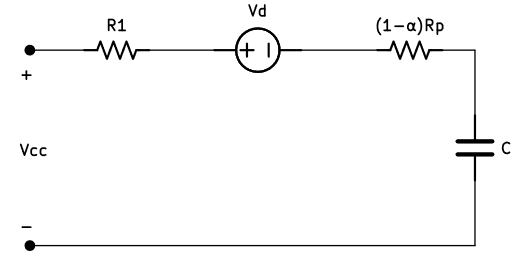
\includegraphics[scale=1]{figure8}
 		\caption{Circuito equivalente para determinar el tiempo de carga tomando en cuenta el modelo del diodo.}
 		\label{fig:pic8}
 	\end{figure}
 
 	En esta ocasión
 	\begin{subequations}
 		\label{E:eq18}
 		\begin{align}
 			v(\infty) &= V_{cc} - V_D\\
 			v(0) &= \frac{V_{cc}}{3}
 		\end{align}
 	\end{subequations}
 
 	Sustituimos la ecuación (\ref{E:eq18}) en la ecuación (\ref{E:eq2})
 	\begin{align}
 		\label{E:eq19}
 		V_c(t) = V_{cc} - V_D + \left[ \frac{V_{cc}}{3} - (V_{cc} - V_D) \right] e^{-\frac{t}{\tau}}
 	\end{align}
 
 	Donde
 	\begin{equation}
 		\label{E:eq20}
 		\tau = R_{eq}C = [R_1 + (1 - \alpha)R_p]C
 	\end{equation}
 
 	El capacitor se cargará hasta que alcance un voltaje igual a $\frac{2V_{cc}}{3}$ por lo tanto
 	\begin{align}
 		\frac{2V_{cc}}{3} &= V_{cc} - V_D + \left[ \frac{V_{cc}}{3} - (V_{cc} - V_D) \right] e^{-\frac{t}{\tau}}\nonumber \\
 		\frac{2V_{cc}}{3} - V_{cc} + V_D &= \left[ \frac{V_{cc}}{3} - V_{cc}  + V_D\right]e^{-\frac{t}{\tau}}\nonumber \\
 		V_D - \frac{V_{cc}}{3} &= \left( V_D - \frac{2V_{cc}}{3} \right)e^{-\frac{t}{\tau}}\nonumber \\
 		e^{-\frac{t}{\tau}} &= \frac{V_D - \frac{V_{cc}}{3}}{V_D - \frac{2V_{cc}}{3}}\nonumber
 	\end{align}
 
 	Por lo tanto
 	\begin{align}
 		\label{E:eq21}
 		t_c = C[R_1 + (1 - \alpha)R_p]\ln \left| \frac{V_D - \frac{V_{cc}}{3}}{V_D - \frac{2V_{cc}}{3}} \right|
 	\end{align}
 
 	\noindent\textbf{Determinando el tiempo de $t_d$}\\\\
 	El circuito equivalente para el tiempo de descarga se muestra en la figura \ref{fig:pic9}
 	\begin{figure}[H]
 		\centering
 		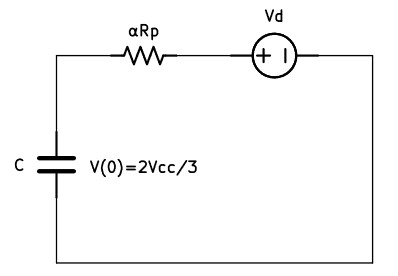
\includegraphics[scale=1]{figure9}
 		\caption{Circuito equivalente para determinar el tiempo de descarga tomando en cuenta el modelo del diodo.}
 		\label{fig:pic9}
 	\end{figure}
 
 	Tenemos que
 	\begin{subequations}
 		\label{E:eq22}
 		\begin{align}
 			v(0) &= \frac{2V_{cc}}{3}\\
 			v(\infty) &= V_D
 		\end{align}
 	\end{subequations}
 
 	Al sustituir la ecuación (\ref{E:eq22}) en la ecuación (\ref{E:eq3}) tenemos 
 	\begin{align}
 		\label{E:eq23}
 		v_c(t) = V_D + (\frac{2V_{cc}}{3} - V_D)e^{-\frac{t}{\tau}}
 	\end{align}
 
 	Donde
 	\begin{align}
 		\label{E:eq24}
 		v_c(t) = V_D + \left(\frac{2V_{cc}}{3} - V_D\right)e^{-\frac{t}{\tau}}
 	\end{align}
 
 	El capacitor se descargará hasta que alcance un valor de $\frac{V_{cc}}{3}$. Así
 	\begin{align}
 		\frac{V_{cc}}{3} = V_D + \left(\frac{2V_{cc}}{3} - V_D\right)e^{-\frac{t}{\tau}}\nonumber \\
 		\frac{V_{cc}}{3} - V_D = \left(\frac{2V_{cc}}{3} - V_D\right)e^{-\frac{t}{\tau}}\nonumber \\
 		\frac{\frac{V_{cc}}{3} - V_D}{\frac{2V_{cc}}{3} - V_D} = e^{-\frac{t}{\tau}}\nonumber
 	\end{align}
 	
 	Así, el tiempo de descarga es
 	\begin{align}
 		\label{E:eq25}
 		t_d = \alpha R_p C \ln(2) \left| \frac{\frac{V_{cc}}{3} - V_D}{\frac{2V_{cc}}{3} - V_D} \right|
 	\end{align}
 
 	El periodo se obtiene de la suma de las ecuaciones (\ref{E:eq21}) y (\ref{E:eq25}), así
 	\begin{align}
 		T = t_c + t_d = C[R_1 + (1 - \alpha)R_p]\ln \left| \frac{V_D - \frac{V_{cc}}{3}}{V_D - \frac{2V_{cc}}{3}} \right| + \alpha R_p C \ln(2) \left| \frac{\frac{V_{cc}}{3} - V_D}{\frac{2V_{cc}}{3} - V_D} \right| \nonumber
 	\end{align}
	\begin{align}
		T = \ln \left| \frac{V_D - \frac{V_{cc}}{3}}{V_D - \frac{2V_{cc}}{3}} \right| [C(R_1 + (1 - \alpha))R_p + \alpha R_p C]\nonumber
	\end{align} 
	\begin{align}
		T = C\ln \left| \frac{V_D - \frac{V_{cc}}{3}}{V_D - \frac{2V_{cc}}{3}} \right| [(R_1 + (1 - \alpha))R_p + \alpha R_p ]\nonumber
	\end{align}
	\begin{align}
		\label{E:eq26}
		T = C(R_1 + R_p)\ln \left| \frac{V_D - \frac{V_{cc}}{3}}{V_D - \frac{2V_{cc}}{3}} \right|
	\end{align}

	\newpage
	
	\begin{myexample}
		Diseñe un circuito PWM a una frecuencia de 100 Hz. Asuma que $C=0.1\mu F$
		\begin{figure}[H]
			\centering
			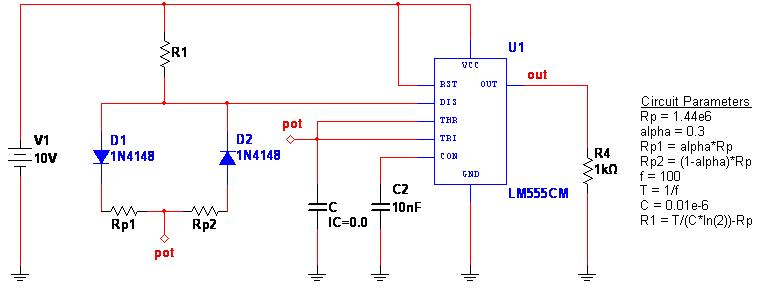
\includegraphics[scale=1]{figure10}
			\caption{Circuito PWM}
			\label{fig:pic10}
		\end{figure}
	
		De la ecuación (\ref{E:eq13}) despejamos el valor de $R_1 + R_p$, por lo tanto
		\begin{align}
			R_1 + R_p &= \frac{T}{C\ln(2)} = \frac{1}{fC\ln(2)}\nonumber \\
			R_1 + R_p &= \frac{1}{(100)(0.1 \times 10^{-6})\ln(2)} = 144.27 k\Omega\nonumber
		\end{align}
	
		Asumiendo un valor comercial para el potenciómetro de $100k\Omega$ tenemos que
		\begin{align}
			R_1 = \frac{1}{fC\ln(2)} - R_p = 44.27 k\Omega \nonumber
		\end{align}
	\end{myexample}

	
 	%\cite{textbook}
	%\bibliographystyle{plain}
	%\bibliography{citation.bib}
	
\end{document}